\section{Substitutionschiffer}
\label{sec:Substitution}
I ett \emph{substitutionschiffer}\index{substitutionschiffer} avbildas varje 
bokstav i klartextalfabetet på en unik bokstav i kryptoalfabetet.
Caesarchiffret är alltså ett substitutionschiffer.
I dagstidningar, bland korsorden, brukar det finnas en typ av korsord som 
kallas för krypto, där rutorna är markerade med tal och varje tal motsvarar en 
bokstav.
Här används alltså det vanliga alfabetet, \(a, b, c, \cdots\), som 
klartextalfabete och talen \(1,2,3,\ldots, 29\) som kryptoalfabete.
Nyckeln i substitutionschiffret utgör hela avbildningen mellan klartext- och 
kryptoalfabetet.
Ett exempel visas i \cref{tbl:Substitutionschiffer}.

\begin{table*}
  \caption{%
    Tabell för att kryptera med ett substitutionschiffer.
		Gemener används som klartextalfabete och versaler som kryptoalfabete.
  }\label{tbl:Substitutionschiffer}
	\centering
	\begin{tabular}{ccccccccccccccc}
    \toprule
    a & b & c & d & e & f & g & h & i & j & k & l & m & n & o \\
		C & M & Q & F & Z & Ö & I & J & P & L & D & N & O & K & D \\
    \midrule
    p & q & r & s & t & u & v & w & x & y & z & å & ä & ö \\
		R & S & T & Å & V & Y & X & W & G & U & Ä & H & A & B \\
    \bottomrule
  \end{tabular}
\end{table*}

För att kryptera gör man på samma sätt som i Caesarchiffret.

\begin{example}\label{ex:SubstitutionHej}
  För att kryptera klartexten \emph{hej} slår man upp bokstav för bokstav 
  i \cref{tbl:Substitutionschiffer}.
	Det vill säga, \(h\mapsto J\), \(e\mapsto Z\) och 
	\(j\mapsto L\).
	Kryptotexten blir alltså \emph{JZL}.
\end{example}

\begin{example}\label{ex:SubstitutionSkatten}
	Om vi krypterar ordet \emph{skatten} blir det \emph{ÅDCVVZK}.
\end{example}

\subsection{Formell definition av substitutionsciffer}
Vi definierar substitutionschiffret som följer.
För enkelthet använder vi samma alfabet för både klartext och kryptotext, även 
om detta inte är en nödvändig begränsning.
Om vi vill ha ett annat kryptoalfabet är detta egentligen bara en fråga om 
kodning, och detta kan läggas till i efterhand.
\begin{definition}[Substitutionschiffer]\label{def:substitutionCipher}\index{substitutionschiffer!formell 
    definition}
  Låt \(A\) vara vårt alfabet och låt \(\P = \C = A\).
  Vidare låt \(\K\) bestå av alla möjliga permutationer av \(A\).
  För varje permutation \(\pi\in \K\) definierar vi att
  \begin{align}
    \nonumber
    e_\pi(p) &= \pi(p), \text{\ och\ } \\
    \nonumber
    d_\pi(c) &= \pi^{-1}(c),
  \end{align}
  där \(\pi^{-1}\) är den inverterade permutationen \(\pi\), \(p\in \P\) är en 
  klartextbokstav och \(c = e_\pi(p)\in \C\) är motsvarande kryptotextbokstav.
\end{definition}

Notera skillnaden mellan användningen av permutationen \(\pi\) i denna 
definition och den i \cref{def:permutationCipher}.
I den tidigare användes permutationen på index i ett block medan i denna 
definition används permutationen direkt på enskilda tecken.
Här permuteras bokstaven medan i den tidigare permuterades bokstavens position.

Vi förtydligar definitionen med följande exempel.
\begin{example}
  Vi kan här återanvända \cref{ex:SubstitutionHej}.
  Vi låter \(A\) vara det svenska alfabetet.
  Nyckeln \(\pi\in \K\) kan vi låta vara densamma som 
  i \cref{ex:SubstitutionHej}, vilken vi ser 
  i \cref{tbl:Substitutionschiffer}.
  Då får vi att \(e_\pi(h) = J, e_\pi(e) = Z, e_\pi(j) = L\).
\end{example}

Värt att notera är att antalet möjliga nycklar \(|\K| = {|A|!}\) växer snabbt 
med storleken av alfabetet.

\begin{exercise}
  Undersök vad som händer vid sammansättning av permutationer i detta chiffer.
  Exempelvis om permutationen \(\pi\) i \cref{def:substitutionCipher} 
  appliceras två gånger, eller att två olika permutationer kombineras: spelar 
  det då någon roll i vilken ordning de appliceras?
\end{exercise}
\begin{exercise}
  Försök att finna en kryptotext \(c\) och två nycklar, \(k\) och \(k^\prime\), 
  sådana att \(d_k(c)\) och \(d_{k^\prime}(c)\) ger tolkningsbara klartexter då 
  med detta kryptosystem.
\end{exercise}

\subsection{Kryptanalys av substitutionschiffer}
\label{sec:KryptanalysSubstitution}
\index{substitutionschiffer!kryptanalys}
För generella substitutionschiffer finns det väsentligen fler möjliga nycklar 
än de 29 möjligheter som fanns för Caesarchiffret, men till kostnad av en 
längre nyckel som är svårare att memorera.
Som första bokstav i nyckeln kan vi välja mellan alla 29 bokstäverna i 
alfabetet.
För varje bokstav vi kan välja som första bokstav finns det 28 bokstäver kvar 
som då kan välja mellan.
Vi får således \[29! = 29\cdot 28\cdot 27\cdots 3\cdot 2\cdot 1 =
8841761993739701954543616000000\] möjliga nycklar\footnote{%
  \({29!}\) uttalas \emph{29 fakultet}.
}, vilket gör det svårt att testa alla möjliga nycklar som vi kunde göra med 
Caesarchiffret.
Vi behöver alltså en annan metod.

Vi analyserar följande text: \enquote{An English text has no Swedish letters}.
Vi vill nu beräkna sannolikheten att välja en specifik bokstav om vi väljer en 
slumpmässig bokstav i denna mening.
Det vill säga, vi väljer en slumpmässig bokstav från mängden
\begin{align}
  \nonumber
  A = \{a, n, e, g, l, i, s, h, t, x, o, w, d, r\}.
\end{align}
Låt \(\x\) beteckna en stockastisk variabel som antar värden ur \(A\).
Vi vet från sannolikhetsläran att sannolikheten \(\Pr(\x = a)\) att vi väljer 
\emph{a} och att detta värde beräknas som
\begin{equation}
  \nonumber
  \Pr(\x = \alpha) = \frac{\#\alpha}{N},
\end{equation}
där \(\#\alpha\) är antalet förkomster av \(\alpha\) i texten och \(N\) är 
totala antalet tecken i texten.
Vi kan då beräkna att \(\Pr(\x = a) = 0.0625\) och alltså att sannolikheten att 
en slumpvis vald bokstav i texten är ett \emph{a} är 6.25 procent.
Värdena av \(\Pr(\x = \alpha)\) för samtliga värden av \(\alpha\) ges 
i \cref{tbl:SannolikhetstabellKlartext}.

\begin{table*}
  \caption{%
    Tabell av sannolikhetsfördelningen för den stokastiska variabeln \(\x\) som 
    antar bokstäver i meningen \enquote{anenglishtexthasnoswedishletters}, 
    angiven med tre decimalers noggrannhet.
  }\label{tbl:SannolikhetstabellKlartext}
	\centering
  \begin{tabular}{rcccccccccc}
    \toprule
    \(\alpha\) & a & b & c & d & e & f & g & h & i & j  \\
    \(\Pr(\x = \alpha)\) & 0.063  & 0.000 & 0.000 & 0.031 & 0.156 & 0.000 
    & 0.031 & 0.094 & 0.064 & 0.000 \\
    \midrule
    \(\alpha\) & k & l & m & n & o & p & q & r & s & t \\
    \(\Pr(\x = \alpha)\) & 0.000 & 0.063 & 0.000 & 0.094 & 0.031 & 0.000 
    & 0.000 & 0.031 & 0.156 & 0.125 \\
    \midrule
    \(\alpha\) & u & v & w & x & y & z & å & ä & ö \\
    \(\Pr(\x = \alpha)\) & 0.000 & 0.000 & 0.031 & 0.031 & 0.000 & 0.000 
    & 0.000 & 0.000 & 0.000 \\
    \bottomrule
  \end{tabular}
\end{table*}
\begin{table*}
  \caption{%
    Tabell av sannolikhetsfördelningen för den stokastiska variabeln \(\y\) som 
    antar bokstäver i meningen \enquote{CPGPINKUJVGZVJCUPQUYGFKUJNGVVGTU}, 
    angiven med tre decimalers noggrannhet.
  }\label{tbl:SannolikhetstabellKryptotext}
	\centering
  \begin{tabular}{rcccccccccccc}
    \toprule
    \(\alpha\) & A & B & C & D & E & F & G & H & I & J \\
    \(\Pr(\y = \alpha)\) & 0.000 & 0.000 & 0.063  & 0.000 & 0.000 & 0.031 
    & 0.156 & 0.000 & 0.031 & 0.094 \\
    \midrule
    \(\alpha\) & K & L & M & N & O & P & Q & R & S & T \\
    \(\Pr(\y = \alpha)\) & 0.064 & 0.000 & 0.000 & 0.063 & 0.000 & 0.094 
    & 0.031 & 0.000 & 0.000 & 0.031 \\
    \midrule
    \(\alpha\) & U & V & W & X & Y & Z & Å & Ä & Ö \\
    \(\Pr(\y = \alpha)\) & 0.156 & 0.125 & 0.000 & 0.000 &  0.031 & 0.031 
    & 0.000 & 0.000 & 0.000 \\
    \bottomrule
  \end{tabular}
\end{table*}

Om vi krypterar en text med ett substitutionschiffer, exempelvis ett 
Caesarchiffer, då förändrar vi inte antalet av någon bokstav, det enda vi 
ändrar är bokstavens representation (''utseende'').
Vi krypterar \enquote{anenglishtexthasnoswedishletters} med något okänt 
substitutionschiffer och får då
\begin{quote}
  CPGPINKUJVGZVJCUPQUYGFKUJNGVVGTU\@.
\end{quote}
Vi låter den stokastiska variabeln \(\y\) anta bokstäver i meningen ovan.
Sannolikhetsfördelningen för \(\y\) är tabellerad 
i \cref{tbl:SannolikhetstabellKryptotext}.
Om vi tittar i tabellen ser vi att \(\Pr(\x = a) = \Pr(\y = C) = \Pr(\y = N)\), 
då har vi alltså två alternativ som skulle kunna representera \emph{a} 
i kryptoalfabetet.
Ett bra riktmärke kan vara att titta på den vanligaste bokstaven, 
i klartextalfabetet är det \emph{e} med \(\Pr(\x = e) = 0.156\).
Det är då mycket möjligt att \(e\mapsto G\) eftersom att \(\Pr(\y = G)\) också 
är \(0.156\).
Ytterligare information vi kan använda är återupprepningar hos bokstäver,
jämför med \cref{ex:CaesarSkatten} och~\ref{ex:SubstitutionSkatten}
där t:et i ordet \emph{skatten} upprepar sig.
De enda bokstäver som upprepar sig i svenskan är konsonanter, och bokstäverna 
omkring dessa är oftast vokaler.
Av vad vi sett hittills verkar det som att kryptotexten är krypterad med ett 
Caesarchiffer med nyckeln C eftersom att \(a\mapsto C\) och \(e\mapsto G\) är 
troliga avbildningar.
Om vi testar att avkryptera enligt Caesarchiffret med nyckeln C ser vi att vår 
gissning var korrekt.

Nu kände vi till sannolikhetsfunktionen för klartexten när vi tittade på
kryptotexten, men hur gör man egentligen när man inte vet någonting om 
klartexten?
Om man har tillräckligt mycket text kommer sannolikhetsfunktionen för texten att 
närma sig sannolikhetsfunktionen för språket.
Då kan textens sannolikhetsfunktion jämföras för att först se vilket språk 
texten är skriven på och därefter kan man hitta nyckeln som vi gjorde ovan.
Sannolikhetsfunktionen för språken svenska och engelska finns givna i 
\cref{tbl:SannolikhetstabellSpråk}.
En överblicksbild för det engelska språket ges även 
i \cref{fig:SannolikhetstabellEngelska}.
Sannolikhetstabeller för några olika språk finns tillgängliga hos 
\cite{Wikipedia2013lf}.

\begin{table*}
  \caption{%
    Tabell av sannolikhetsfördelningen för bokstäver i det 
    engelska~\cite{Stinson2006cta} och det svenska~\cite{Wikipedia2013lf} 
    språket, den stokastiska variabeln \(\e\) respektive \(\s\), angiven med 
    tre decimalers noggrannhet.
  }\label{tbl:SannolikhetstabellSpråk}
	\centering
  \begin{tabular}{rcccccccccc}
    \toprule
    \(\alpha\) & a & b & c & d & e & f & g & h & i & j \\
    \(\Pr(\e = \alpha)\) & 0.082  & 0.015 & 0.028 & 0.043 & 0.127 & 0.022 
    & 0.020 &
    0.061 & 0.070 & 0.002 \\
    \(\Pr(\s = \alpha)\) & 0.093  & 0.013 & 0.013 & 0.045 & 0.099 & 0.020 
    & 0.033 &
		0.021 & 0.051 & 0.007 \\
    \midrule
    \(\alpha\) & k & l & m & n & o & p & q & r & s & t \\
    \(\Pr(\e = \alpha)\) & 0.008 & 0.040 & 0.024 & 0.067 & 0.075 & 0.019 
    & 0.001 & 0.060 & 0.063 & 0.091 \\
    \(\Pr(\s = \alpha)\) & 0.032 & 0.052 & 0.035 & 0.088 & 0.041 & 0.017 
    & 0.000 & 0.083 & 0.063 & 0.087 \\
    \midrule
    \(\alpha\) & u & v & w & x & y & z & å & ä & ö \\
    \(\Pr(\e = \alpha)\) & 0.028 & 0.010 & 0.023 & 0.001 & 0.020 & 0.001 
    & 0.000 & 0.000 & 0.000 \\
    \(\Pr(\s = \alpha)\) & 0.018 & 0.024 & 0.000 & 0.001 & 0.006 & 0.000 
    & 0.016 & 0.021 & 0.015 \\
    \bottomrule
  \end{tabular}
\end{table*}

\begin{figure*}
	\centering
  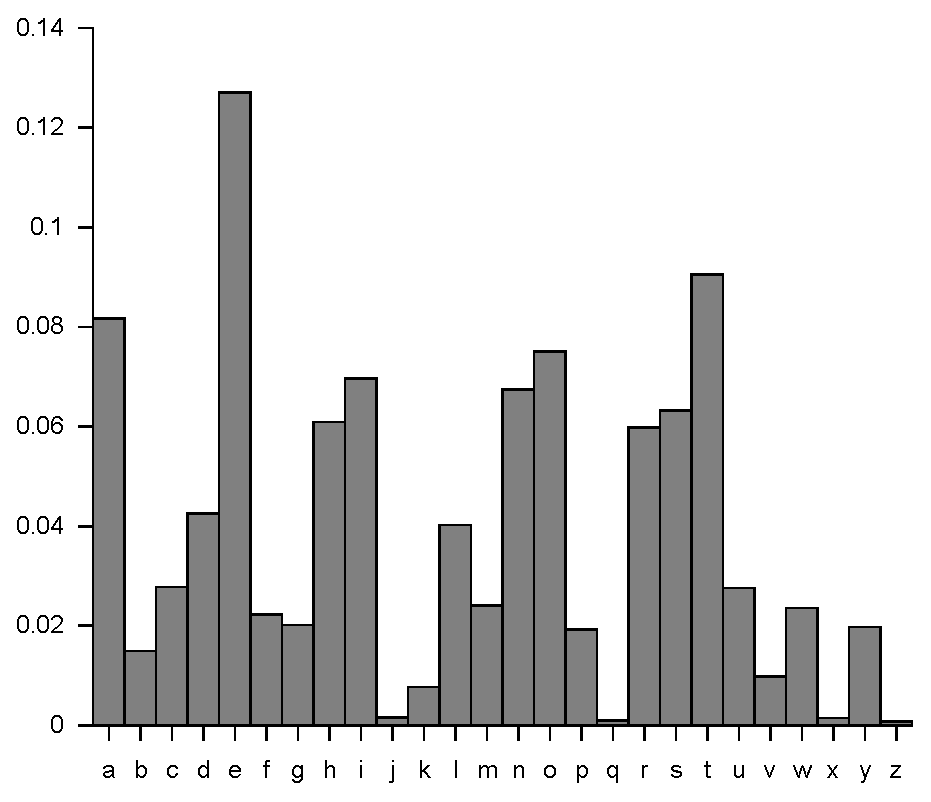
\includegraphics[width=0.7\linewidth]{figs/english_letter_frequencies.eps}
  \caption{%
    En överblickande graf över sannolikhetsfördelningen för den stokastiska 
    variabeln \(\e\).
    Bild:~\cite{Wikipedia2013lf}.
  }\label{fig:SannolikhetstabellEngelska}
\end{figure*}

\begin{exercise}
  Du jobbar som kryptoanalytiker åt Försvarets Radioanstalt (FRA) och får 
  följande text på ditt skrivbord:
  % XXX rewrite plaintext examples to Swedish
	\begin{verbatim}
    VJGOCFJCVVGTUVGCRCTVUWPFGTYC
    KVKUKPVJGWUWCNRNCEGDGJKPFVJGEWTVCKP
  \end{verbatim}
  \begin{comment}
  \begin{verbatim}
    THN MJNSXNGKD RM PNTTNJW AG TNZT HUW RMTNG CNNG WTXVANV MRJ XWN AG
    KJDQTRIJUQHD, UGV MJNSXNGKD UGUPDWAW AG QUJTAKXPUJ. GR NZUKT PNTTNJ
    MJNSXNGKD VAWTJACXTARG XGVNJPANW U IAYNG PUGIXUIN, WAGKN UPP EJATNJW
    EJATN WPAIHTPD VAMMNJNGTPD. PAGRTDQN FUKHAGNW WRJTNV THN PNTTNJW'
    MJNSXNGKANW UW NTURAG WHJVPX KFMEDQ YCIOSL ZB CUWNV RG THN NZQNJANGKN
    UGV KXWTRF RM FUGXUP KRFQRWATRJW. PAONEAWN, FRVNJG AGTNJGUTARGUP FRJWN
    KRVN NGKRVNW THN FRWT MJNSXNGT PNTTNJW EATH THN WHRJTNWT WDFCRPW;
    UJJUGIAGI THN FRJWN UPQHUCNT AGTR IJRXQW RM PNTTNJW THUT JNSXAJN NSXUP
    UFRXGTW RM TAFN TR TJUGWFAT, UGV THNG WRJTAGI THNWN IJRXQW AG
    AGKJNUWAGI RJVNJ, DANPVW N AT WUG HXJVF EIYPMCO RQLZKB DS. WAFAPUJ
    AVNUW UJN XWNV AG FRVNJG VUTU-KRFQJNWWARG TNKHGASXNW WXKH UW HXMMFUG
    KRVAGI.
  \end{verbatim}
	\end{comment}
	Vad betyder det?

	\begin{comment}
		För att knäcka krypteringen gör man en frekvensanalys av bokstäverna.
		Bokstavsfrekvenser för olika språk finns på
		\begin{center}
			\url{http://en.wikipedia.org/wiki/Letter_frequency#Relative_frequencies_of_letters_in_the_English_language}.
		\end{center}

		Det krypterade meddelandet är
		\begin{quote}
      the mad hatter's teaparty is underway\@. it is in the usual place,
			behind the curtain.
		\end{quote}
		\begin{quotation}\noindent
      the frequency of letters in text has often been studied for use in 
      cryptography, and frequency analysis in particular\@. no exact letter 
      frequency distribution underlies a given language, since all writers 
      write slightly differently\@. linotype machines sorted the letters' 
      frequencies as etaoin shrdlu cmfwyp vbgkqj xz based on the experience and 
      custom of manual compositors\@. likewise, modern international morse code 
      encodes the most frequent letters with the shortest symbols; arranging 
      the morse alphabet into groups of letters that require equal amounts of 
      time to transmit, and then sorting these groups in increasing order, 
      yields e it san hurdm wgvlfbk opjxcz yq\@. similar ideas are used in 
      modern data-compression techniques such as huffman coding.
		\end{quotation}
		Det har krypterats med ett substitutionschiffer som har nyckeln
		\begin{verbatim}
      UCKVNMIHALOPFGRQSJWTXYEZDB.
    \end{verbatim}
	\end{comment}
\end{exercise}

